% This file was created by tikzplotlib v0.8.1.
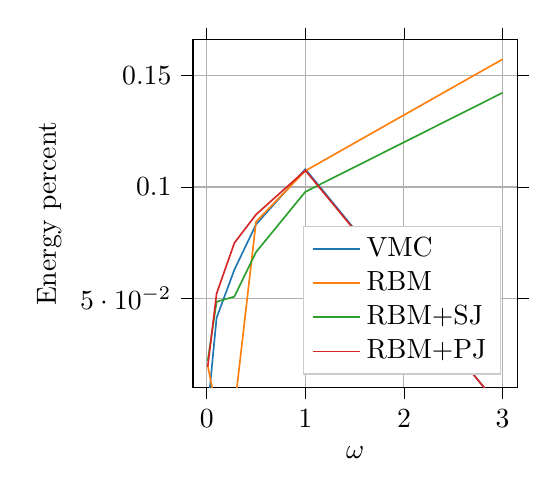
\begin{tikzpicture}

\definecolor{color0}{rgb}{0.12156862745098,0.466666666666667,0.705882352941177}
\definecolor{color1}{rgb}{1,0.498039215686275,0.0549019607843137}
\definecolor{color2}{rgb}{0.172549019607843,0.627450980392157,0.172549019607843}
\definecolor{color3}{rgb}{0.83921568627451,0.152941176470588,0.156862745098039}

\begin{axis}[
legend cell align={left},
legend style={at={(0.34,0.465)}, 
anchor=north west, 
draw=white!80.0!black},
tick align=outside,
tick pos=both,
x grid style={white!69.01960784313725!black},
xlabel={\(\displaystyle \omega\)},
xmajorgrids,
xmin=-0.1395, 
xmax=3.1495,
width=5.7cm,
height=6cm,
xtick style={color=black},
y grid style={white!69.01960784313725!black},
%ylabel={\(\displaystyle \langle\mathcal{T}\rangle/\langle\mathcal{H}\rangle\)},
ylabel={Energy percent},
ymajorgrids,
ymin=0.01, ymax=0.166,
ytick style={color=black}
]
\addplot [semithick, color0]
table {%
0.01 0
0.1 0.041314897
0.28 0.062858938
0.5 0.083185086
1 0.108006304
3 0
};
\addlegendentry{VMC}
\addplot [semithick, color1]
table {%
0.01 0.019880972
0.1 0
0.28 0
0.5 0.084401654
1 0.107237934
3 0.157246497
};
\addlegendentry{RBM}
\addplot [semithick, color2]
table {%
0.01 0.021990704
0.1 0.048556688
0.28 0.050807505
0.5 0.070803652
1 0.097821651
3 0.142231886
};
\addlegendentry{RBM+SJ}
\addplot [semithick, color3]
table {%
0.01 0.019452496
0.1 0.052195251
0.28 0.074859347
0.5 0.087636916
1 0.10741901
3 0
};
\addlegendentry{RBM+PJ}
\end{axis}

\end{tikzpicture}